\documentclass[]{article}
\usepackage{lmodern}
\usepackage{amssymb,amsmath}
\usepackage{ifxetex,ifluatex}
\usepackage{fixltx2e} % provides \textsubscript
\ifnum 0\ifxetex 1\fi\ifluatex 1\fi=0 % if pdftex
\usepackage[T1]{fontenc}
\usepackage[utf8]{inputenc}
\else % if luatex or xelatex
\ifxetex
\usepackage{mathspec}
\else
\usepackage{fontspec}
\fi
\defaultfontfeatures{Ligatures=TeX,Scale=MatchLowercase}
\fi
% use upquote if available, for straight quotes in verbatim environments
\IfFileExists{upquote.sty}{\usepackage{upquote}}{}
% use microtype if available
\IfFileExists{microtype.sty}{%
    \usepackage[]{microtype}
    \UseMicrotypeSet[protrusion]{basicmath} % disable protrusion for tt fonts
}{}
\PassOptionsToPackage{hyphens}{url} % url is loaded by hyperref
\usepackage[unicode=true]{hyperref}
\hypersetup{
    pdftitle={Rapport projet base de données - Rapizz},
    pdfauthor={Romain Gille Erwan Maugere},
    pdfborder={0 0 0},
    breaklinks=true}
\urlstyle{same}  % don't use monospace font for urls
\usepackage[margin=1in]{geometry}
\usepackage{color}
\usepackage{fancyvrb}
\newcommand{\VerbBar}{|}
\newcommand{\VERB}{\Verb[commandchars=\\\{\}]}
\DefineVerbatimEnvironment{Highlighting}{Verbatim}{commandchars=\\\{\}}
% Add ',fontsize=\small' for more characters per line
\newenvironment{Shaded}{}{}
\newcommand{\KeywordTok}[1]{\textcolor[rgb]{0.00,0.44,0.13}{\textbf{#1}}}
\newcommand{\DataTypeTok}[1]{\textcolor[rgb]{0.56,0.13,0.00}{#1}}
\newcommand{\DecValTok}[1]{\textcolor[rgb]{0.25,0.63,0.44}{#1}}
\newcommand{\BaseNTok}[1]{\textcolor[rgb]{0.25,0.63,0.44}{#1}}
\newcommand{\FloatTok}[1]{\textcolor[rgb]{0.25,0.63,0.44}{#1}}
\newcommand{\ConstantTok}[1]{\textcolor[rgb]{0.53,0.00,0.00}{#1}}
\newcommand{\CharTok}[1]{\textcolor[rgb]{0.25,0.44,0.63}{#1}}
\newcommand{\SpecialCharTok}[1]{\textcolor[rgb]{0.25,0.44,0.63}{#1}}
\newcommand{\StringTok}[1]{\textcolor[rgb]{0.25,0.44,0.63}{#1}}
\newcommand{\VerbatimStringTok}[1]{\textcolor[rgb]{0.25,0.44,0.63}{#1}}
\newcommand{\SpecialStringTok}[1]{\textcolor[rgb]{0.73,0.40,0.53}{#1}}
\newcommand{\ImportTok}[1]{#1}
\newcommand{\CommentTok}[1]{\textcolor[rgb]{0.38,0.63,0.69}{\textit{#1}}}
\newcommand{\DocumentationTok}[1]{\textcolor[rgb]{0.73,0.13,0.13}{\textit{#1}}}
\newcommand{\AnnotationTok}[1]{\textcolor[rgb]{0.38,0.63,0.69}{\textbf{\textit{#1}}}}
\newcommand{\CommentVarTok}[1]{\textcolor[rgb]{0.38,0.63,0.69}{\textbf{\textit{#1}}}}
\newcommand{\OtherTok}[1]{\textcolor[rgb]{0.00,0.44,0.13}{#1}}
\newcommand{\FunctionTok}[1]{\textcolor[rgb]{0.02,0.16,0.49}{#1}}
\newcommand{\VariableTok}[1]{\textcolor[rgb]{0.10,0.09,0.49}{#1}}
\newcommand{\ControlFlowTok}[1]{\textcolor[rgb]{0.00,0.44,0.13}{\textbf{#1}}}
\newcommand{\OperatorTok}[1]{\textcolor[rgb]{0.40,0.40,0.40}{#1}}
\newcommand{\BuiltInTok}[1]{#1}
\newcommand{\ExtensionTok}[1]{#1}
\newcommand{\PreprocessorTok}[1]{\textcolor[rgb]{0.74,0.48,0.00}{#1}}
\newcommand{\AttributeTok}[1]{\textcolor[rgb]{0.49,0.56,0.16}{#1}}
\newcommand{\RegionMarkerTok}[1]{#1}
\newcommand{\InformationTok}[1]{\textcolor[rgb]{0.38,0.63,0.69}{\textbf{\textit{#1}}}}
\newcommand{\WarningTok}[1]{\textcolor[rgb]{0.38,0.63,0.69}{\textbf{\textit{#1}}}}
\newcommand{\AlertTok}[1]{\textcolor[rgb]{1.00,0.00,0.00}{\textbf{#1}}}
\newcommand{\ErrorTok}[1]{\textcolor[rgb]{1.00,0.00,0.00}{\textbf{#1}}}
\newcommand{\NormalTok}[1]{#1}
\usepackage{graphicx,grffile}
\makeatletter
\def\maxwidth{\ifdim\Gin@nat@width>\linewidth\linewidth\else\Gin@nat@width\fi}
\def\maxheight{\ifdim\Gin@nat@height>\textheight\textheight\else\Gin@nat@height\fi}
\makeatother
% Scale images if necessary, so that they will not overflow the page
% margins by default, and it is still possible to overwrite the defaults
% using explicit options in \includegraphics[width, height, ...]{}
\setkeys{Gin}{width=\maxwidth,height=\maxheight,keepaspectratio}
\IfFileExists{parskip.sty}{%
    \usepackage{parskip}
}{% else
    \setlength{\parindent}{0pt}
    \setlength{\parskip}{6pt plus 2pt minus 1pt}
}
\setlength{\emergencystretch}{3em}  % prevent overfull lines
\providecommand{\tightlist}{%
    \setlength{\itemsep}{0pt}\setlength{\parskip}{0pt}}
\setcounter{secnumdepth}{0}
% Redefines (sub)paragraphs to behave more like sections
\ifx\paragraph\undefined\else
\let\oldparagraph\paragraph
\renewcommand{\paragraph}[1]{\oldparagraph{#1}\mbox{}}
\fi
\ifx\subparagraph\undefined\else
\let\oldsubparagraph\subparagraph
\renewcommand{\subparagraph}[1]{\oldsubparagraph{#1}\mbox{}}
\fi

% set default figure placement to htbp
\makeatletter
\def\fps@figure{htbp}
\makeatother


\title{Rapport projet base de données - Rapizz}
\author{Romain Gille Erwan Maugere}
\date{\today}

\begin{document}
\maketitle

{
    \setcounter{tocdepth}{3}
    \tableofcontents
}
\newpage

\section{Le projet et ses
    contraintes}\label{le-projet-et-ses-contraintes}

\subsection{Description du projet}\label{description-du-projet}

L'objectif principal visé par ce projet est la conception d'une base de
données permettant de répondre aux besoins exprimés.\\
La base de données développée doit être capable de gérer l'activité
quotidienne de vente et de livraison de Rapizz.\\
La base devra notamment vérifier le solde des comptes utilisateurs
afin de refuser les commandes pour lesquels le solde est insuffisant.\\
La base doit aussi être capable de vérifier le montant de la facture
pour ne pas facturer les pizzas gratuites grâce aux points de fidélité
ou au retard.\\
De plus, la base doit pouvoir proposer un suivi du chiffre d'affaires
des ventes des pizzas et effectuer des statistiques diverses sur les
activités.

\subsection{Contraintes du projet}\label{contraintes-du-projet}

\subsection{Technologies}\label{technologies}

\begin{itemize}
        \tightlist
    \item
        MariaDB FTW
    \item
        mysql-client
    \item
        JMerizzz
    \item
        eclipse \& windowbuilder plugin \& jdbc libs
    \item
        \textbf{DID I MENTION I USE ARCH LINUX ?}
\end{itemize}

\section{La base de données}\label{la-base-de-donnuxe9es}

\subsection{Schemas}\label{schemas}

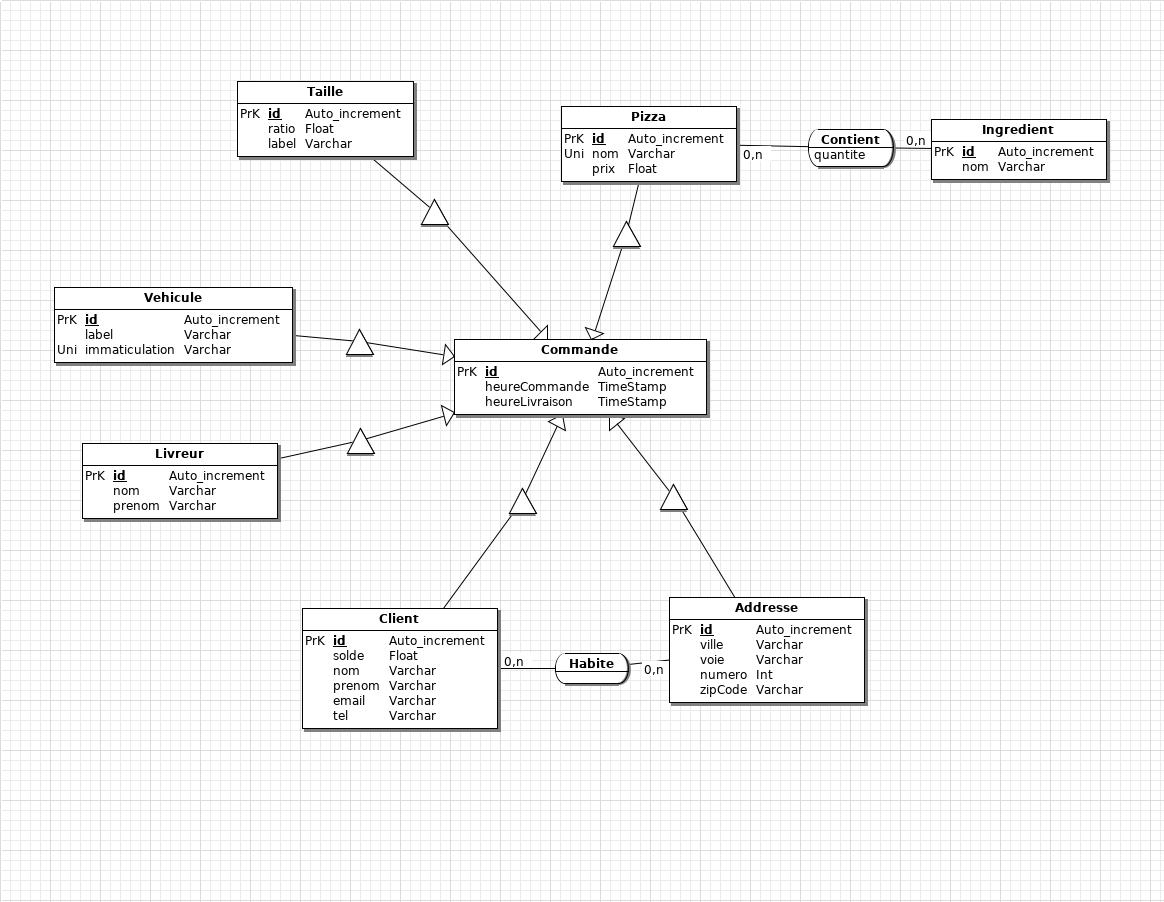
\includegraphics{../img/mcd.jpg} 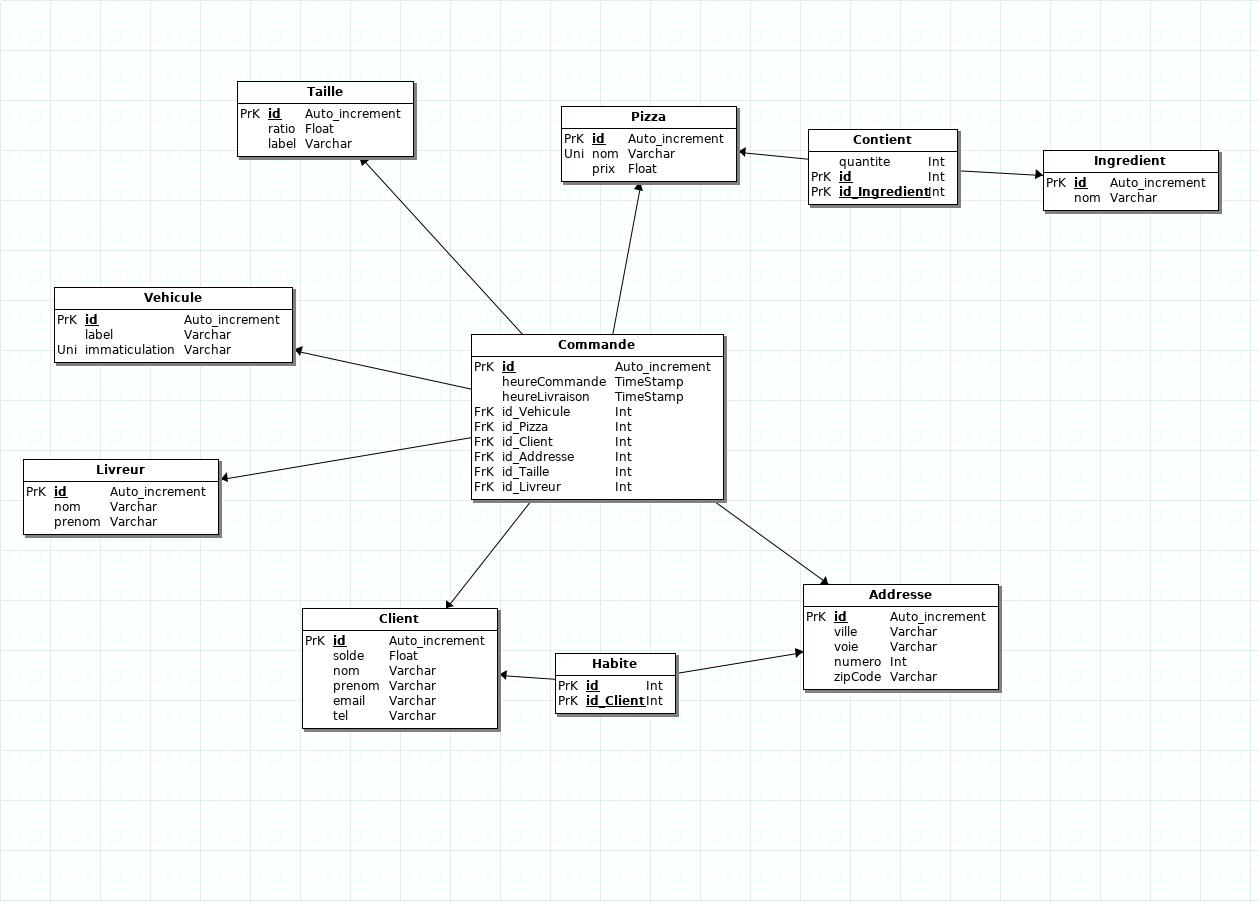
\includegraphics{../img/mld.jpg}

\subsection{Détails}\label{duxe9tails}

\subsubsection{Calcul du prix d'une
    pizza}\label{calcul-du-prix-dune-pizza}

Chaque pizza a un prix de base qui est estimé à partir de la liste des
ingrédients et de la complexité de sa préparation. Ce prix est celui
affiché sur la carte de la pizzeria.\\
Cependant, un second paramètre est à prendre en compte pour obtenir
le prix réel d'une pizza. En effet, il est possible de commander des
pizzas de tailles différentes, la taille portera une influence sur le
prix final de la pizza.\\
Rapizz propose aujourd'hui trois tailles de pizza: l'\textbf{humaine}, la
\textbf{naine} et l'\textbf{ogresse}.\\
La taille dite ``humaine'' est à considérer comme la taille normale et est
proposée par défaut. Cette taille n'influe pas le prix finale de la pizza
(ratio de 1).\\
A contrario, les tailles ``naine'' et ``ogresse'' influent le prix à
hauteur respective d'une diminution et d'une augmentation d'un tier.\\
Pour appliquer ces changements de prix, la table \texttt{Taille} de
notre base de données comporte un champ \texttt{ratio} qui représente
l'influence de la taille sur le prix.\\
Dans la table \texttt{Commande}, une pizza est associée à sa taille.
Il est ainsi possible d'obtenir le prix réel d'une pizza en appliquant le
ratio de la taille sur le prix de base de la pizza.

Cette opération se fait grâce à la requête suivante:

\begin{Shaded}
    \begin{Highlighting}[]
        \KeywordTok{SELECT}
        \NormalTok{p.prix }\KeywordTok{AS} \OtherTok{`prix de base"}\NormalTok{,}
        \NormalTok{    t.ratio }\KeywordTok{AS} \OtherTok{"ratio taille"}\NormalTok{,}
        \NormalTok{    p.prix*t.ratio }\KeywordTok{AS} \OtherTok{"prix reel"}
        \KeywordTok{FROM}\NormalTok{ Commande c}
        \KeywordTok{NATURAL} \KeywordTok{JOIN}\NormalTok{ Pizza p}
        \KeywordTok{NATURAL} \KeywordTok{JOIN}\NormalTok{ Taille t}
        \KeywordTok{WHERE}\NormalTok{ c.id=}\DecValTok{2} \CommentTok{-- id de commande}
        \NormalTok{;}
    \end{Highlighting}
\end{Shaded}

\subsubsection{Calcul du temps de
    livraison}\label{calcul-du-temps-de-livraison}

Notre table \texttt{Commande} est composée de deux champs
\texttt{heureCommande} et \texttt{heureLivraison} de type Timestamp qui
représentent repectivement les dates et heures de commande et de
livraison.\\
Le champ \texttt{heureLivraison} est un champ qui peut être
\texttt{null} ce qui permet de ne le saisir qu'après la livraison
effective de la commande.

On peut alors, grâce à la requête suivante obtenir le temps de livraison
d'une commande:

\begin{Shaded}
    \begin{Highlighting}[]
        \KeywordTok{SELECT}
        \NormalTok{    heureCommande,}
        \NormalTok{    heureLivraison,}
        \NormalTok{    heureCommande - heureLivraison }\KeywordTok{AS} \OtherTok{"temps de livraison"}
        \KeywordTok{FROM}\NormalTok{ Commande}
        \KeywordTok{WHERE}\NormalTok{ id=}\DecValTok{1} \CommentTok{-- id de commande}
        \NormalTok{;}
    \end{Highlighting}
\end{Shaded}

\newpage

\subsubsection{Pizza de fidélite
    offerte}\label{pizza-de-fiduxe9lite-offerte}

La pizzeria Rapizz a une offre de fidelité pour ses clients. Au bout de
dix commandes, la pizza est offerte.\\
Pour vérifier si une commande doit être offerte, il faut suivre une
procédure en deux étapes : calculer le nombre de commandes d'un client,
puis, vérifier si la commande est un chiffre rond.

Calcul du nombre de commandes par client:

\begin{Shaded}
    \begin{Highlighting}[]
        \KeywordTok{SELECT}
        \NormalTok{    clt.nom,}
        \FunctionTok{COUNT}\NormalTok{(cmd.id_Client) }\KeywordTok{AS} \OtherTok{"nb Commandes"}
        \KeywordTok{FROM}\NormalTok{ Commande cmd}
        \KeywordTok{NATURAL} \KeywordTok{JOIN}\NormalTok{ Client clt}
        \KeywordTok{GROUP} \KeywordTok{BY}\NormalTok{ clt.nom;}
    \end{Highlighting}
\end{Shaded}

Il nous suffit ensuite de faire un modulo \(10\) et de vérifier si il
vaut \(0\).

\subsubsection{Adresse de clients et adresse de
    livraison}\label{adresse-de-clients-et-adresse-de-livraison}

Un client a la possibilité de saisir différentes adresses de livraison.
Cette fonctionnalité est incorporée à notre base de donnée par l'usage
d'une table de liaison entre les tables \texttt{Client} et
\texttt{Adresse}.\\
Chaque commande doit aussi être liée à une adresse d'où la présence d'une clé
étrangère \texttt{id\_Adresse}.

\subsection{Procédures}\label{procuxe9dures}

\begin{Shaded}
    \begin{Highlighting}[]
        \KeywordTok{CREATE} \KeywordTok{PROCEDURE}\NormalTok{ AjoutIngredient (}\KeywordTok{IN}\NormalTok{ ingredient }\DataTypeTok{VARCHAR}\NormalTok{(}\DecValTok{25}\NormalTok{)) MODIFIES SQL }\KeywordTok{DATA}
        \KeywordTok{BEGIN}
        \KeywordTok{INSERT} \KeywordTok{INTO}\NormalTok{ Ingredient (nom) }\FunctionTok{VALUE}\NormalTok{ (ingredient);}
        \NormalTok{END}

        \KeywordTok{CREATE} \KeywordTok{PROCEDURE}\NormalTok{ AjoutLivreur (}\KeywordTok{IN}\NormalTok{ nom }\DataTypeTok{VARCHAR}\NormalTok{(}\DecValTok{25}\NormalTok{), prenom }\DataTypeTok{VARCHAR}\NormalTok{(}\DecValTok{25}\NormalTok{)) MODIFIES SQL }\KeywordTok{DATA}
        \KeywordTok{BEGIN}
        \KeywordTok{INSERT} \KeywordTok{INTO}\NormalTok{ Livreur (nom, prenom) }\FunctionTok{VALUE}\NormalTok{ (nom, prenom);}
        \NormalTok{END}

        \KeywordTok{CREATE} \KeywordTok{PROCEDURE}\NormalTok{ AjoutVehicule (}\KeywordTok{IN} \KeywordTok{label} \DataTypeTok{VARCHAR}\NormalTok{(}\DecValTok{25}\NormalTok{), immat }\DataTypeTok{VARCHAR}\NormalTok{(}\DecValTok{25}\NormalTok{)) MODIFIES SQL }\KeywordTok{DATA}
        \KeywordTok{BEGIN}
        \KeywordTok{INSERT} \KeywordTok{INTO}\NormalTok{ Vehicule (}\KeywordTok{label}\NormalTok{, immatriculation) }\FunctionTok{VALUE}\NormalTok{ (}\KeywordTok{label}\NormalTok{, immat);}
        \NormalTok{END}
    \end{Highlighting}
\end{Shaded}

\subsubsection{SYSTEM FEATURES}\label{system-features}

\begin{itemize}
        \tightlist
    \item
        check client solde
    \item
        get client bill
    \item
        check for free pizza
    \item
        check free pizza by exceed delivery time
    \item
        find best client
    \item
        find the worst deliveryman
    \item
        find best/worst pizza
    \item
        find best ingredient
\end{itemize}

\subsubsection{MENU}\label{menu}

\begin{itemize}
        \tightlist
    \item
        find data to print menu
    \item
        list pizza, price, ingredients, \ldots{}
\end{itemize}

\subsubsection{DELIVERY BILL}\label{delivery-bill}

\begin{itemize}
        \tightlist
    \item
        find data to print delivery bill
    \item
        blablabla
\end{itemize}

\subsubsection{RANDOM REQUESTS}\label{random-requests}

\begin{itemize}
        \tightlist
    \item
        find vehicle never used
    \item
        calculate amount of order by client
    \item
        calculate average of orders
    \item
        find clients with more ordres than avg
\end{itemize}

\newpage

\section{Interface graphique}\label{interface-graphique}

\begin{figure}[!htb]
    \minipage{0.5\textwidth}
    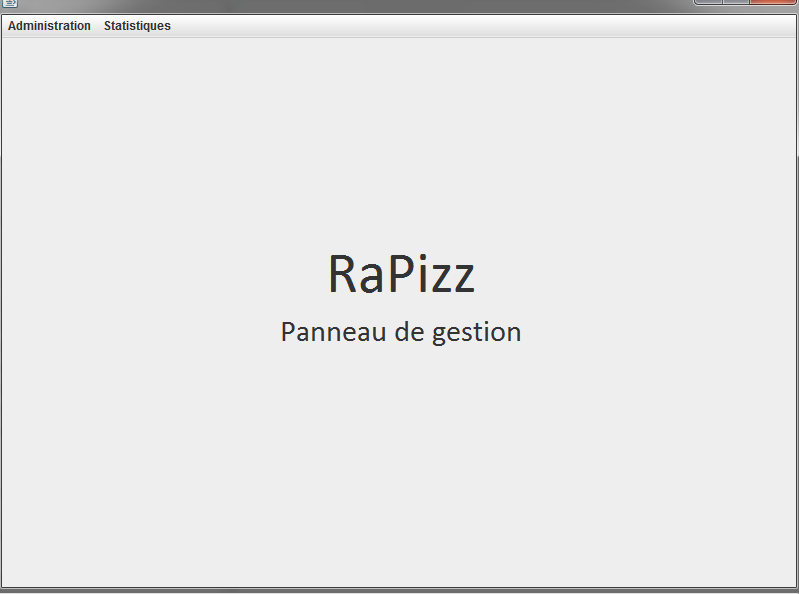
\includegraphics{../img/ihm/accueil.png}
\endminipage\hfill
\minipage{0.5\textwidth}
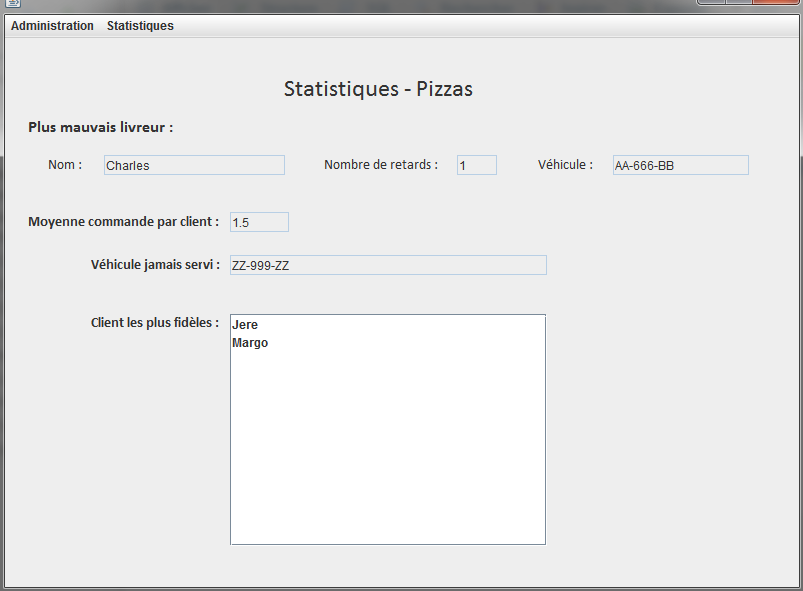
\includegraphics{../img/ihm/stats.png}
\endminipage\hfill
\end{figure}

\begin{figure}[!htb]
    \minipage{0.5\textwidth}
    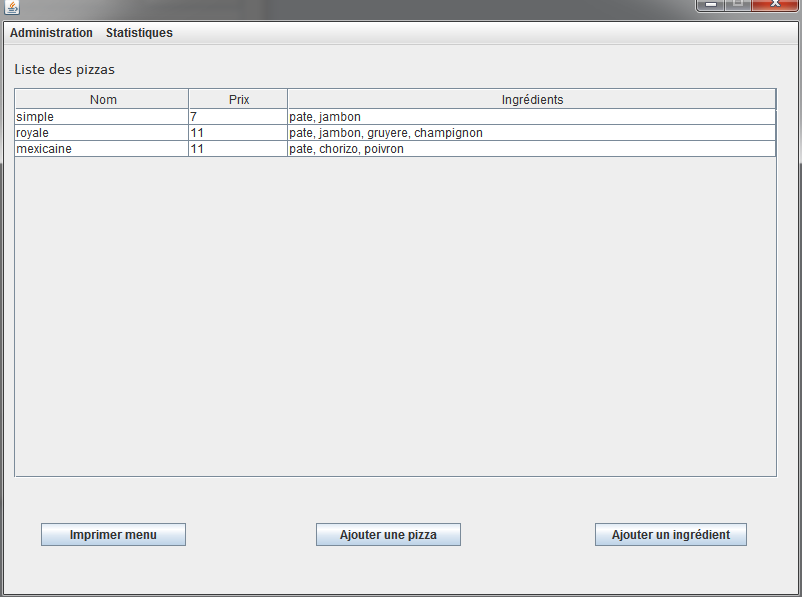
\includegraphics{../img/ihm/liste_pizza.png}
\endminipage\hfill
\minipage{0.5\textwidth}
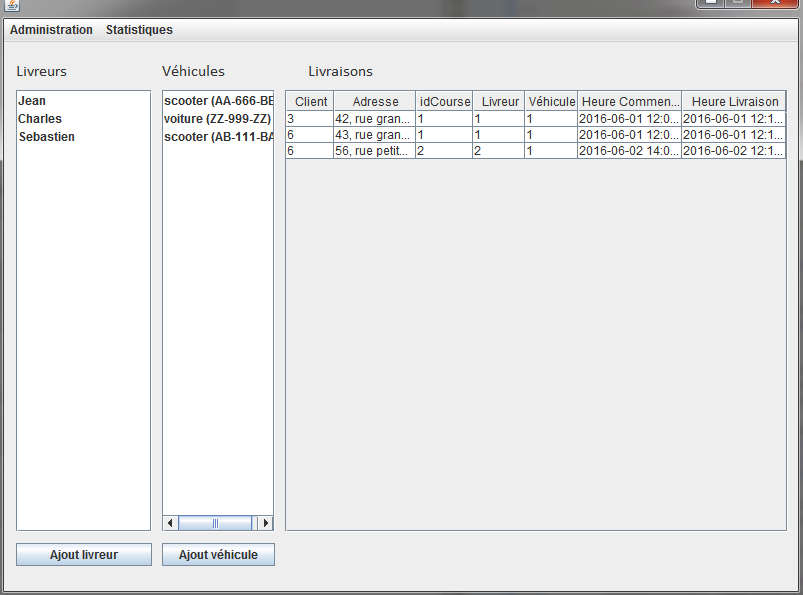
\includegraphics{../img/ihm/3emescreen.png}
\endminipage\hfill
\end{figure}

\begin{figure}[!htb]
    \minipage{0.5\textwidth}
    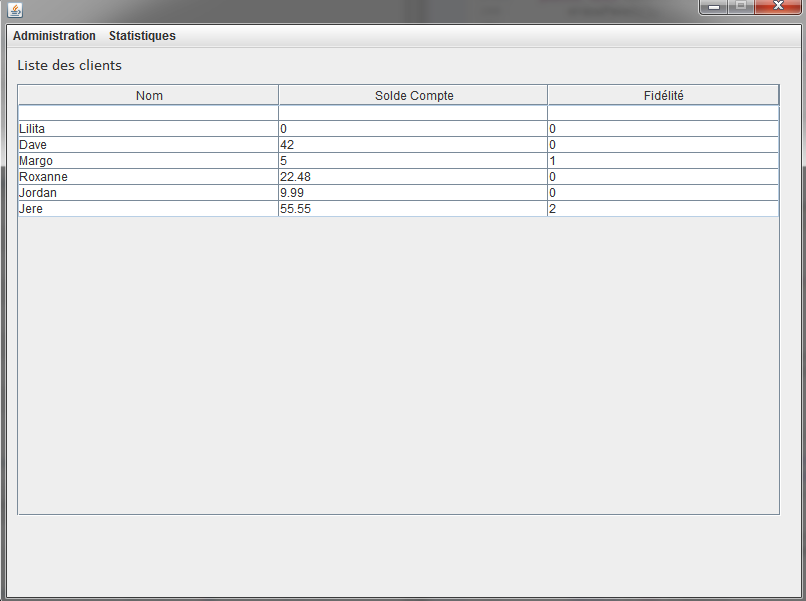
\includegraphics{../img/ihm/liste_clients.png}
\endminipage\hfill
\end{figure}


\section{Conclusion}\label{conclusion}

Ce projet nous a permis d'approfondir nos connaissances en base de données,
en IHM mais également en Markdown et en LaTeX pour le rapport.

\section{Annexes}\label{annexes}

Script de création de la base de donnée:

\href{../../script/create.sql}{create.sql}

Script d'insertion d'un jeu de données de test:

\href{../../script/insert.sql}{insert.sql}

Procedures usuelles:

\href{../../script/procedures.sql}{procedures.sql}

\end{document}
